% Options for packages loaded elsewhere
\PassOptionsToPackage{unicode}{hyperref}
\PassOptionsToPackage{hyphens}{url}
%
\documentclass[
]{article}
\usepackage{amsmath,amssymb}
\usepackage{lmodern}
\usepackage{ifxetex,ifluatex}
\ifnum 0\ifxetex 1\fi\ifluatex 1\fi=0 % if pdftex
  \usepackage[T1]{fontenc}
  \usepackage[utf8]{inputenc}
  \usepackage{textcomp} % provide euro and other symbols
\else % if luatex or xetex
  \usepackage{unicode-math}
  \defaultfontfeatures{Scale=MatchLowercase}
  \defaultfontfeatures[\rmfamily]{Ligatures=TeX,Scale=1}
\fi
% Use upquote if available, for straight quotes in verbatim environments
\IfFileExists{upquote.sty}{\usepackage{upquote}}{}
\IfFileExists{microtype.sty}{% use microtype if available
  \usepackage[]{microtype}
  \UseMicrotypeSet[protrusion]{basicmath} % disable protrusion for tt fonts
}{}
\makeatletter
\@ifundefined{KOMAClassName}{% if non-KOMA class
  \IfFileExists{parskip.sty}{%
    \usepackage{parskip}
  }{% else
    \setlength{\parindent}{0pt}
    \setlength{\parskip}{6pt plus 2pt minus 1pt}}
}{% if KOMA class
  \KOMAoptions{parskip=half}}
\makeatother
\usepackage{xcolor}
\IfFileExists{xurl.sty}{\usepackage{xurl}}{} % add URL line breaks if available
\IfFileExists{bookmark.sty}{\usepackage{bookmark}}{\usepackage{hyperref}}
\hypersetup{
  pdftitle={XXX},
  hidelinks,
  pdfcreator={LaTeX via pandoc}}
\urlstyle{same} % disable monospaced font for URLs
\usepackage[margin=1in]{geometry}
\usepackage{graphicx}
\makeatletter
\def\maxwidth{\ifdim\Gin@nat@width>\linewidth\linewidth\else\Gin@nat@width\fi}
\def\maxheight{\ifdim\Gin@nat@height>\textheight\textheight\else\Gin@nat@height\fi}
\makeatother
% Scale images if necessary, so that they will not overflow the page
% margins by default, and it is still possible to overwrite the defaults
% using explicit options in \includegraphics[width, height, ...]{}
\setkeys{Gin}{width=\maxwidth,height=\maxheight,keepaspectratio}
% Set default figure placement to htbp
\makeatletter
\def\fps@figure{htbp}
\makeatother
\setlength{\emergencystretch}{3em} % prevent overfull lines
\providecommand{\tightlist}{%
  \setlength{\itemsep}{0pt}\setlength{\parskip}{0pt}}
\setcounter{secnumdepth}{-\maxdimen} % remove section numbering
\usepackage{setspace}\doublespacing
\usepackage{lineno}\linenumbers
\usepackage{booktabs}
\usepackage{longtable}
\usepackage{array}
\usepackage{multirow}
\usepackage{wrapfig}
\usepackage{float}
\usepackage{colortbl}
\usepackage{pdflscape}
\usepackage{tabu}
\usepackage{threeparttable}
\usepackage{threeparttablex}
\usepackage[normalem]{ulem}
\usepackage{makecell}
\usepackage{xcolor}
\ifluatex
  \usepackage{selnolig}  % disable illegal ligatures
\fi
\newlength{\cslhangindent}
\setlength{\cslhangindent}{1.5em}
\newlength{\csllabelwidth}
\setlength{\csllabelwidth}{3em}
\newenvironment{CSLReferences}[2] % #1 hanging-ident, #2 entry spacing
 {% don't indent paragraphs
  \setlength{\parindent}{0pt}
  % turn on hanging indent if param 1 is 1
  \ifodd #1 \everypar{\setlength{\hangindent}{\cslhangindent}}\ignorespaces\fi
  % set entry spacing
  \ifnum #2 > 0
  \setlength{\parskip}{#2\baselineskip}
  \fi
 }%
 {}
\usepackage{calc}
\newcommand{\CSLBlock}[1]{#1\hfill\break}
\newcommand{\CSLLeftMargin}[1]{\parbox[t]{\csllabelwidth}{#1}}
\newcommand{\CSLRightInline}[1]{\parbox[t]{\linewidth - \csllabelwidth}{#1}\break}
\newcommand{\CSLIndent}[1]{\hspace{\cslhangindent}#1}

\title{XXX}
\author{}
\date{\vspace{-2.5em}}

\begin{document}
\maketitle

\begin{center}
\textbf{ORDER TBD:  H{\'{e}}ctor Tejero-Cicu{\'{e}}ndez$^{1,*}$,  Iris Men{\'{e}}ndez$^{2,3}$, Salvador Carranza$^{1}$, and Dean C. Adams$^{4}$} 
\end{center}

\begin{center}22 September, 2022\end{center}

\(^{1}\)Institute of Evolutionary Biology (CSIC-Universitat Pompeu
Fabra), Passeig Marítim de la Barceloneta 37-49, Barcelona 08002, Spain

\(^{2}\)Departamento de Geodinámica, Estratigrafía y Paleontología,
Facultad de Ciencias Geológicas, Universidad Complutense de Madrid,
C/José Antonio Novais 12, Madrid 28040, Spain

\(^{3}\)Departamento de Cambio Medioambiental, Instituto de Geociencias
(UCM, CSIC), C/Severo Ochoa 7, Madrid 28040, Spain

\(^{4}\)Department of Ecology, Evolution, and Organismal Biology, Iowa
State University, Ames, Iowa, 50010 USA

\(^{*}\)Correspondence: Héctor Tejero-Cicuéndez
\href{mailto:cicuendez93@gmail.com}{\nolinkurl{cicuendez93@gmail.com}}

\hfill\break

\textbf{Keywords}: Phenotypic Evolution, Morphospace, Allometry,
\emph{Pristurus} geckos \hfill\break

\textbf{Short Title}: XXX \hfill\break

\textbf{Author Contributions}: All authors collaboratively developed the
concept and contributed to all portions of this manuscript. HT-C, IM,
and DCA performed the analyses. All authors approve of the final product
and are willingly accountable for any portion of the
content.\hfill\break

\textbf{Conflicts of Interests}: The authors declare no conflicts of
interest.\hfill\break

\textbf{Data Archiving}: Data are available on DRYAD
(\url{doi:10.5061/dryad.xwdbrv1f6} (Tejero-Cicuéndez et al. 2021b)).
R-scripts are available at \textbf{XXX}. \hfill\break

\textbf{Acknowledgments}: We thank XYZPDQ\ldots{} This work was
sponsored in part by XXX (to SC) DCA was funded in part by National
Science Foundation Grant DEB-2140720, and a Fulbright Senior Scholar
Grant.

\newpage

\hypertarget{abstract}{%
\section{Abstract}\label{abstract}}

asdf

\newpage

\hypertarget{introduction}{%
\section{Introduction}\label{introduction}}

The mechanisms through which phenotypic diversity emerges and evolves
are an essential topic of study in evolutionary biology. Such diversity
is the result of a combination of genetic, developmental, and
environmental factors that determine the life history of organisms and
the evolutionary trajectory of species. These factors might impose
certain constraints or offer opportunities for morphological evolution,
generating the diversity upon which natural selection acts culminating
in the adaptation of species to their surrounding environments.
Consequently, the differences in species' ecological preferences (e.g.,
the exploitation of different habitats) have the potential to drive
morphological changes via distinct selective pressures. \hfill\break

Ecological specialization is one of the main sources of phenotypic
diversity. When organisms colonize new and unique habitats, they are
subjected to novel ecological dynamics that may impose different
functional requirements. This ecomorphological relationship may result
in the repeated evolution of certain phenotypes (i.e., convergence) and
the appearance of the so-called ecomorphs, when the general
morphological features of the species within a clade can be tightly
related to specific ecological contexts. This includes emblematic
examples of adaptive radiations such as the differential body size and
shape of Anolis species exploiting different microhabitats (Losos 2009),
the disparity in beak morphology in Darwin's finches (REFS) and Hawaiian
honeycreepers (REFS), or the differences in jaw morphology among cichlid
fishes (REFS). \hfill\break

However, while the patterns of morphological differences among distinct
ecological contexts have been well documented in a variety of vertebrate
taxa, the specific trajectories of morphological evolution are in many
cases less known. A particularly interesting question is perhaps the
extent to which evolutionary allometry can describe this phenotypic
differentiation. ALLOMETRY BLABLABLA. \hfill\break

The Afro-Arabian geckos in the genus \emph{Pristurus} afford the
opportunity to elucidate the interdigitating effects of allometry and
habitat specialization on clade-level patterns of phenotypic diversity.
Prior work on this system (Tejero-Cicuéndez et al. 2021a) revealed that
the colonization of ground habitats has been a trigger of morphological
change, specifically reflected in an increase in body size and shape
disparity. Interestingly, some ground-dwelling species are among the
largest of the genus and also show increased relative head sizes and
limb proportions, while some other species with this ecological
specialization have evolved to be among the smallest of the group.
Additionally, among the species exploiting rocky habitats (the most
common ecological feature in \emph{Pristurus}), there are also species
with both considerably large and small body sizes (Tejero-Cicuéndez et
al. 2021a). What remains unexplored, however, is how the evolution of
body shape is related to differences in body size and whether habitat
specialization has an impact in this relationship shape-size. (how this
relationship shape-size differs among habitats.) \hfill\break

\textbf{last paragraph} In this study, we used a combination of
multivariate morphometric and phylogenetic comparative analysis to
interrogate macroevolutionary patterns of evolutionary allometry in
\emph{Pristurus} geckos of Afro-Arabia. Using a combination of
phenotypic, phylogenetic, and ecological data, we characterized
allometric trends in body form to discern the extent to which those
patterns differed across species occupying distinct ecological habitats,
and to explore how allometric differences related to overall patterns of
phenotypic diversification in the group.

The independent diversification of both Socotran and continental taxa,
the ecological and behavioural diversity and the unique phenotypic
dataset compiled in this study, make this group of geckos an attractive
model system to investigate keystone dynamics in evolutionary biology
such as the island effect and ecological adaptation, and their impact on
morphological evolution.

Our findings

Overall our work has \ldots{} (some implication).

Our results demonstrate that differing tracectories of allometric growth
can result in similar adult phenotypes\ldots{} (Don't like it! We've got
adults, yes? )

\hypertarget{materials-and-methods}{%
\section{Materials and Methods}\label{materials-and-methods}}

\hypertarget{data}{%
\subsection{Data}\label{data}}

We used a combination of phenotypic, phylogenetic, and ecological data
to characterize and evaluate interspectific allometric trends. The data
utilized here were obtained from our prior work on this system
(Tejero-Cicuéndez et al. 2021a, 2022), and are briefly described here.
First we used a time-dated, molecular phylogeny that included all
members of the genus \emph{Pristurus}, including several currently
undescribed taxa. The tree was estimated in a Bayesian framework, using
five mitochondrial markers, six nuclear markers, and 21 calibration
points (for details see Tejero-Cicuéndez et al. 2022). Next we
categorized each species as belonging to one of three ecological groups
(ground, rock, or tree), based on descriptions of habitat use found in
the literature (see Tejero-Cicuéndez et al. 2021a). Finally, we obtained
a phenotypic data set containing body size (snout-vent length: SVL) and
eight linear measurements (Figure 1) that described overall body form:
trunk length (TrL), head length (HL), head width (HW), head height (HH),
humerus length (Lhu), ulna length (Lun), femur length (Lfe), and tibia
length (Ltb) (Tejero-Cicuéndez et al. 2021a). We restricted our study to
those species represented by five or more individuals; resulting in a
dataset of 687 individuals from 25 species (invidivuals per species:
\(\mu=27\); min = 9, max = 56). Species in the phenotypic dataset were
then matched to the phylogeny, which was subsequently pruned to arrive
at the final topology. All measurements were log-transformed prior to
statistical analyses. Additional details regarding data collection and
formal descriptions of each linear measurement may be found in the
original sources (see Tejero-Cicuéndez et al. 2021a, 2022). The data are
found on DRYAD: \url{https://doi.org/10.5061/dryad.xwdbrv1f6}
(Tejero-Cicuéndez et al. 2021b).

\hypertarget{statistical-and-comparative-analyses}{%
\subsection{Statistical and Comparative
Analyses}\label{statistical-and-comparative-analyses}}

\textbf{EVOLUTIONARY ALLOMETRY} Do just shape \textasciitilde{} size \&
shape \textasciitilde size for species \textbar{} phylogeny

THen mancova\ldots.

\begin{itemize}
\tightlist
\item
  compare habitat slopes we found with individuals to those from species
  means (the `usual' way of looking at evolutionary allometry)
\end{itemize}

We conducted a series of analyses to interrogate allometric trends and
macroevolutionary changes in allometry, relative to diversification in
body form. First, to determine whether allometric trends in body form
differed across habitat groups, we performed a multivariate analysis of
covariance, with body size (\(SVL\)), \(habitat\), and
\(SVL\times habitat\) as model effects. Significance was evaluated using
999 iterations of a permutation procedure, where residuals from a
reduced model were randomly permuted in each permutation (RRPP), model
statistics were recalculated, and used to generate empirical null
sampling distributions to evaluate the observed test statistics
(following Freedman and Lane 1983; Collyer and Adams 2007; Collyer et
al. 2015). Next we compared the multivariate allometric vectors for each
habitat group by calculating pairwise differences in their angular
direction in morphospace, and evaluating these relative to empirical
sampling distributions obtained through RRPP (Collyer and Adams 2007;
Adams and Collyer 2009; Collyer and Adams 2013). We then visualized
patterns of multivariate allometry relative to body size via regression
scores (Drake and Klingenberg 2008) and predicted lines (Adams and
Nistri 2010), based on the coefficients and fitted values from the
linear model described above. \hfill\break

Second, we examined changes in allometric trends across the phylogeny,
treating the head dimensions and limb dimensions separately. Because
both the head and limb data were multivariate, we accomplished this by
first performing a partial least squares analysis (Rohlf and Corti 2000)
of the head traits versus SVL, and the limb traits versus SVL, and
retaining the PLS scores for each individual from the first dimension of
this analysis. Species-specific slopes describing the extent of head and
limb allometry within each species were then obtained from an analysis
of covariance modeled as: \(PLS1_{head} \sim SVL*species\) and
\(PLS1_{limb} \sim SVL*species\) respectively. Species' slopes were then
mapped on the phylogeny of \emph{Pristurus} using a Brownian motion
model of evolution, to qualitatively evaluate shifts in allometry across
species (for a similar approach see Adams and Nistri 2010). \hfill\break

Finally, to relate within-species allometric trends with patterns of
phenotypic diversification in the group we generated a phylomorphospace,
based on the size-standardized species means obtained from a
phylogenetic regression (see Tejero-Cicuéndez et al. 2021a). Here,
phenotypic similarities among species, relative to their phylogenetic
relationships and habitat affiliations, were observed. All analyses were
conducted in R 4.2.1 (R Core Team 2022), using \texttt{RRPP} version
1.3.1 (Collyer and Adams 2018; Collyer and Adams 2022), and scripts
written by the authors (available at \textbf{XXX}).

\hypertarget{results}{%
\section{Results}\label{results}}

Our analyses revealed significant differences in the allometry of body
form among \emph{Pristurus} that utilized distinct habitats (Table 1).
Further, comparisons of multivariate allometric vectors identified that
ground-dwelling \emph{Pristurus} displayed a distinct allometric trend
as compared with \emph{Pristurus} occupying both the rock and tree
habitats (Table 2). A visualization of multivariate allometric trends
(Fig. 2) confirmed these statistical findings, and indicated that the
allometric trajectory in rock-dwelling animals was more extreme as
compared with either ground or tree-dwelling \emph{Pristurus}.
Inspection of individual regression coefficients for each trait
(Supplemental Information) further corroborated this, revealing steeper
allometric coefficients for all head and limb traits in ground-dwelling
\emph{Pristurus} as compared with rock and tree-dwelling taxa. Overall,
these findings revealed that larger individuals of ground-dwelling
\emph{Pristurus} species displayed proportionately larger heads and
limbs, as compared with large individuals in taxa utilizing other
habitat types. \hfill\break

Ground: head and body dimensions are more positively allometric
(relative to SVL) than in rock/tree groups, and whereas allometric
coefficients more similar in rock \& tree.

Formally evaluated using PLS: confirming \ldots\ldots. WHen mapped on
the phylogeny (\ldots.) Here traitgrams (by SVL) elucidated that heads
more strongly allometric in XXX, implying that larger individuals of
these species display proportionately larger heads relative to the
`typical' trend in the genus. By contrast, \ldots{} less strong
(negative? ) allometry

steeper/shallower slopes? resulting in \ldots{}

**Careful! use steeper slope, not positive/negative.

When viewed in light of phylomorphospace\ldots.

\hypertarget{discussion}{%
\section{Discussion}\label{discussion}}

\newpage

\hypertarget{references}{%
\section*{References}\label{references}}
\addcontentsline{toc}{section}{References}

\setlength{\parindent}{-0.25in} \setlength{\leftskip}{0.25in}
\setlength{\parskip}{8pt} \noindent

\hypertarget{refs}{}
\begin{CSLReferences}{1}{0}
\leavevmode\hypertarget{ref-AdamsCollyer2009}{}%
Adams, D. C., and M. L. Collyer. 2009. A general framework for the
analysis of phenotypic trajectories in evolutionary studies. Evolution
63:1143--1154.

\leavevmode\hypertarget{ref-AdamsNistri2010}{}%
Adams, D. C., and A. Nistri. 2010. Ontogenetic convergence and evolution
of foot morphology in european cave salamanders (family:
plethodontidae). BMC Evolutionary Biology 10:1--10. BioMed Central.

\leavevmode\hypertarget{ref-CollyerAdams2007}{}%
Collyer, M. L., and D. C. Adams. 2007. Analysis of two-state
multivariate phenotypic change in ecological studies. Ecology
88:683--692.

\leavevmode\hypertarget{ref-CollyerAdams2013}{}%
Collyer, M. L., and D. C. Adams. 2013. Phenotypic trajectory analysis:
Comparison of shape change patterns in evolution and ecology. Hystrix
24:75--83.

\leavevmode\hypertarget{ref-RRPP}{}%
Collyer, M. L., and D. C. Adams. 2022. R: RRPP: Linear model evaluation
with randomized residuals in a permutation procedure. Vsn. 1.3.1. R
Foundation for Statistical Computing, Vienna, Austria.

\leavevmode\hypertarget{ref-CollyerAdams2018}{}%
Collyer, M. L., and D. C. Adams. 2018. RRPP: An r package for fitting
linear models to high-dimensional data using residual randomization.
Methods in Ecology and Evolution 9:1772--1779.

\leavevmode\hypertarget{ref-Collyer_et_al2015}{}%
Collyer, M. L., D. J. Sekora, and D. C. Adams. 2015. A method for
analysis of phenotypic change for phenotypes described by
high-dimensional data. Heredity 115:357--365.

\leavevmode\hypertarget{ref-DrakeKlingenberg2008}{}%
Drake, A. G., and C. P. Klingenberg. 2008. The pace of morphological
change: Historical transformation of skull shape in st bernard dogs.
Proceedings of the Royal Society B: Biological Sciences 275:71--76.

\leavevmode\hypertarget{ref-Freedman1983}{}%
Freedman, D., and D. Lane. 1983. A nonstochastic interpretation of
reported significance levels. Journal of Business {\&} Economic
Statistics 1:292--298.

\leavevmode\hypertarget{ref-RCT}{}%
R Core Team. 2022. R: A language and environment for statistical
computing. Version 4.2.1. R Foundation for Statistical Computing,
Vienna, Austria.

\leavevmode\hypertarget{ref-Rohlf2000}{}%
Rohlf, F. J., and M. Corti. 2000. Use of two-block partial least-squares
to study covariation in shape. Systematic Biology 49:740--753.

\leavevmode\hypertarget{ref-Tejero-Cicuendez2022}{}%
Tejero-Cicuéndez, H., A. H. Patton, D. S. Caetano, J. Šmíd, L. J.
Harmon, and S. Carranza. 2022. Reconstructing squamate biogeography in
afro-arabia reveals the influence of a complex and dynamic geologic
past. Systematic Biology 71:261--272.

\leavevmode\hypertarget{ref-Tejero-Cicuendez2021}{}%
Tejero-Cicuéndez, H., M. Simó-Riudalbas, I. Menéndez, and S. Carranza.
2021a. Ecological specialization, rather than the island effect,
explains morphological diversification in an ancient radiation of
geckos. Proceedings of the Royal Society B: Biological Sciences
288:20211821.

\leavevmode\hypertarget{ref-PristurusData}{}%
Tejero-Cicuéndez, H., M. Simó-Riudalbas, I. Menéndez, and S. Carranza.
2021b. Ecological specialization, rather than the island effect,
explains morphological diversification in an ancient radiation of
geckos. Dryad digital repository. (Doi:10.5061/dryad.xwdbrv1f6).

\end{CSLReferences}

\newpage

\begin{table}[H]

\caption{\label{tab:unnamed-chunk-1}Multivariate analysis of covariance describing variation in body form in    extit{Pristurus}.}
\centering
\begin{tabular}[t]{llllllll}
\toprule
  & Df & SS & MS & Rsq & F & Z & Pr(>F)\\
\midrule
svl & 1 & 516.036559 & 516.0365588 & 0.9203096 & 10188.69842 & 9.490057 & 0.001\\
habitat & 2 & 6.218510 & 3.1092552 & 0.0110902 & 61.38957 & 9.322480 & 0.001\\
svl:habitat & 2 & 3.974307 & 1.9871536 & 0.0070879 & 39.23464 & 7.077264 & 0.001\\
Residuals & 681 & 34.491245 & 0.0506479 & 0.0615124 &  &  & \\
Total & 686 & 560.720622 &  &  &  &  & \\
\bottomrule
\end{tabular}
\end{table}

\newpage

\begin{table}[H]

\caption{\label{tab:unnamed-chunk-2}Pairwise comparisons of multivariate allometry vectors. Effect sizes ($Z_{\theta_{12}}$) based on pairwise differences in angular direction are below the diagonal, and their corresponding significance levels are above diagonal. Significant values in bold.}
\centering
\begin{tabular}[t]{llll}
\toprule
  & Ground & Rock & Tree\\
\midrule
Ground & 0 & \textbf{0.001} & \textbf{0.001}\\
Rock & \textbf{6.872} & 0 & 0.261\\
Tree & \textbf{3.657} & 0.649 & 0\\
\bottomrule
\end{tabular}
\end{table}

\newpage

\hypertarget{figures}{%
\section{Figures}\label{figures}}

Figure 1. Linear Measurements used in this study. SVL = snout-vent
length, TL = trunk length, HL = head length, HW = head width, HH = head
height, Lhu = humerus length, Lun = ulna length, Lfe = femur length, Ltb
= tibia length (for details see Tejero-Cicuéndez et al. 2021a).
\hfill\break

Figure 2. Plot of regression scores and predicted lines representing the
relationship between linear body measurements and size (SVL).
Individuals re colored by habitat use: rock (beige), ground (dark
purple), and tree (magenta). \hfill\break

Figure 3. Traitgrams showing the evolution of body size (SVL) through
time based on the phylogenetic tree of \emph{Pristurus}. Colors
represent an evolutionary mapping of regression slopes describing the
relationship of (A) head morphology versus body size, and (B) limb
proportions versus body size (see text for descriptions). Species names
are colored by habitat use: rock (beige), ground (dark purple), and tree
(magenta). \hfill\break

Figure 4. Phylomorphospace of \emph{Pristurus}, based on residuals from
a phylogenetic regression of body measurements on size (SVL). Species
means are colored by habitat use: rock (beige), ground (dark purple),
and tree (magenta). Large and small rock-dwelling and ground-dwelling
are highlighted with darker colors to highlight their differentiation
and relative positions in morphospace.

\newpage

\begin{figure}

{\centering 
\includegraphics[width=1\linewidth]{Figs/Fig1} 

}

\caption{Linear Measurements used in this study. SVL = snout-vent length, TL = trunk length, HL = head length, HW = head width, HH = head height, Lhu = humerus length, Lun = ulna length, Lfe = femur length, Ltb = tibia length (for details see Tejero-Cicu{'{e}}ndez et al. 2021a).}\label{fig:unnamed-chunk-3}
\end{figure}

\newpage

\begin{figure}
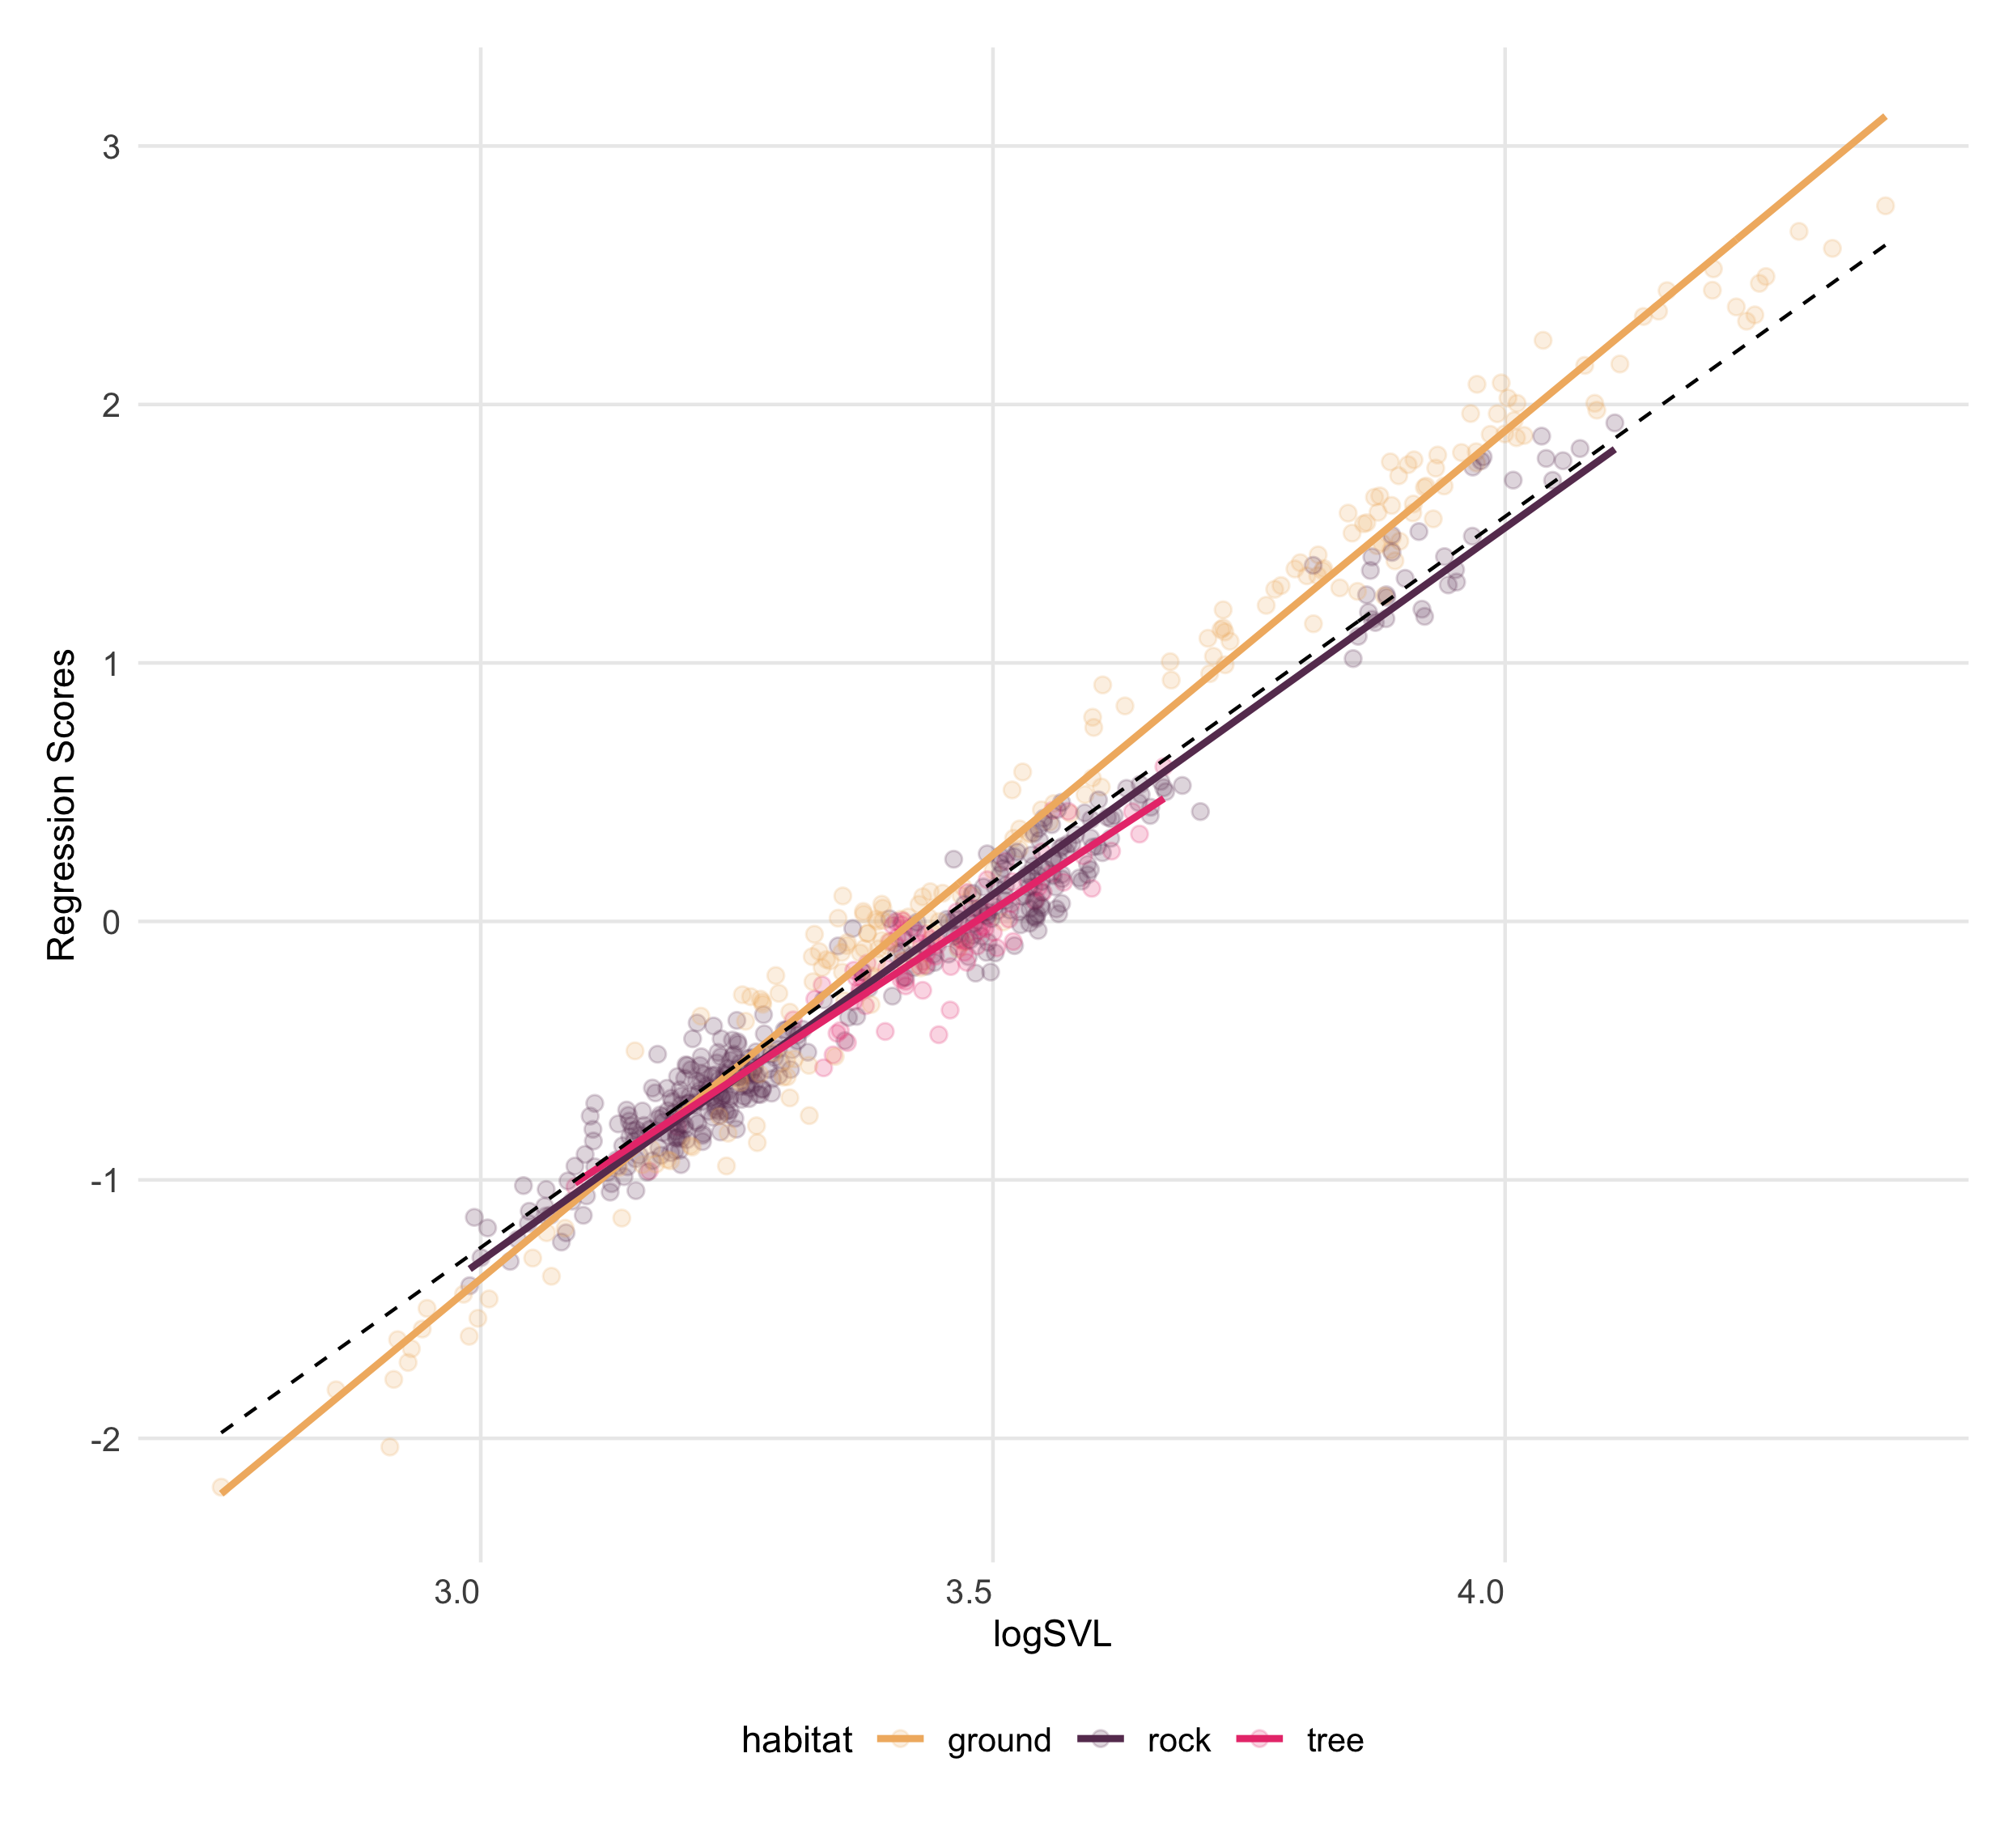
\includegraphics[width=1\linewidth]{Figs/figure_2_ggplot} \caption{Plot of regression scores and predicted lines representing the relationship between linear body measurements and size (SVL). Individuals re colored by habitat use: rock (beige), ground (dark purple), and tree (magenta).}\label{fig:unnamed-chunk-4}
\end{figure}

\newpage

\begin{figure}
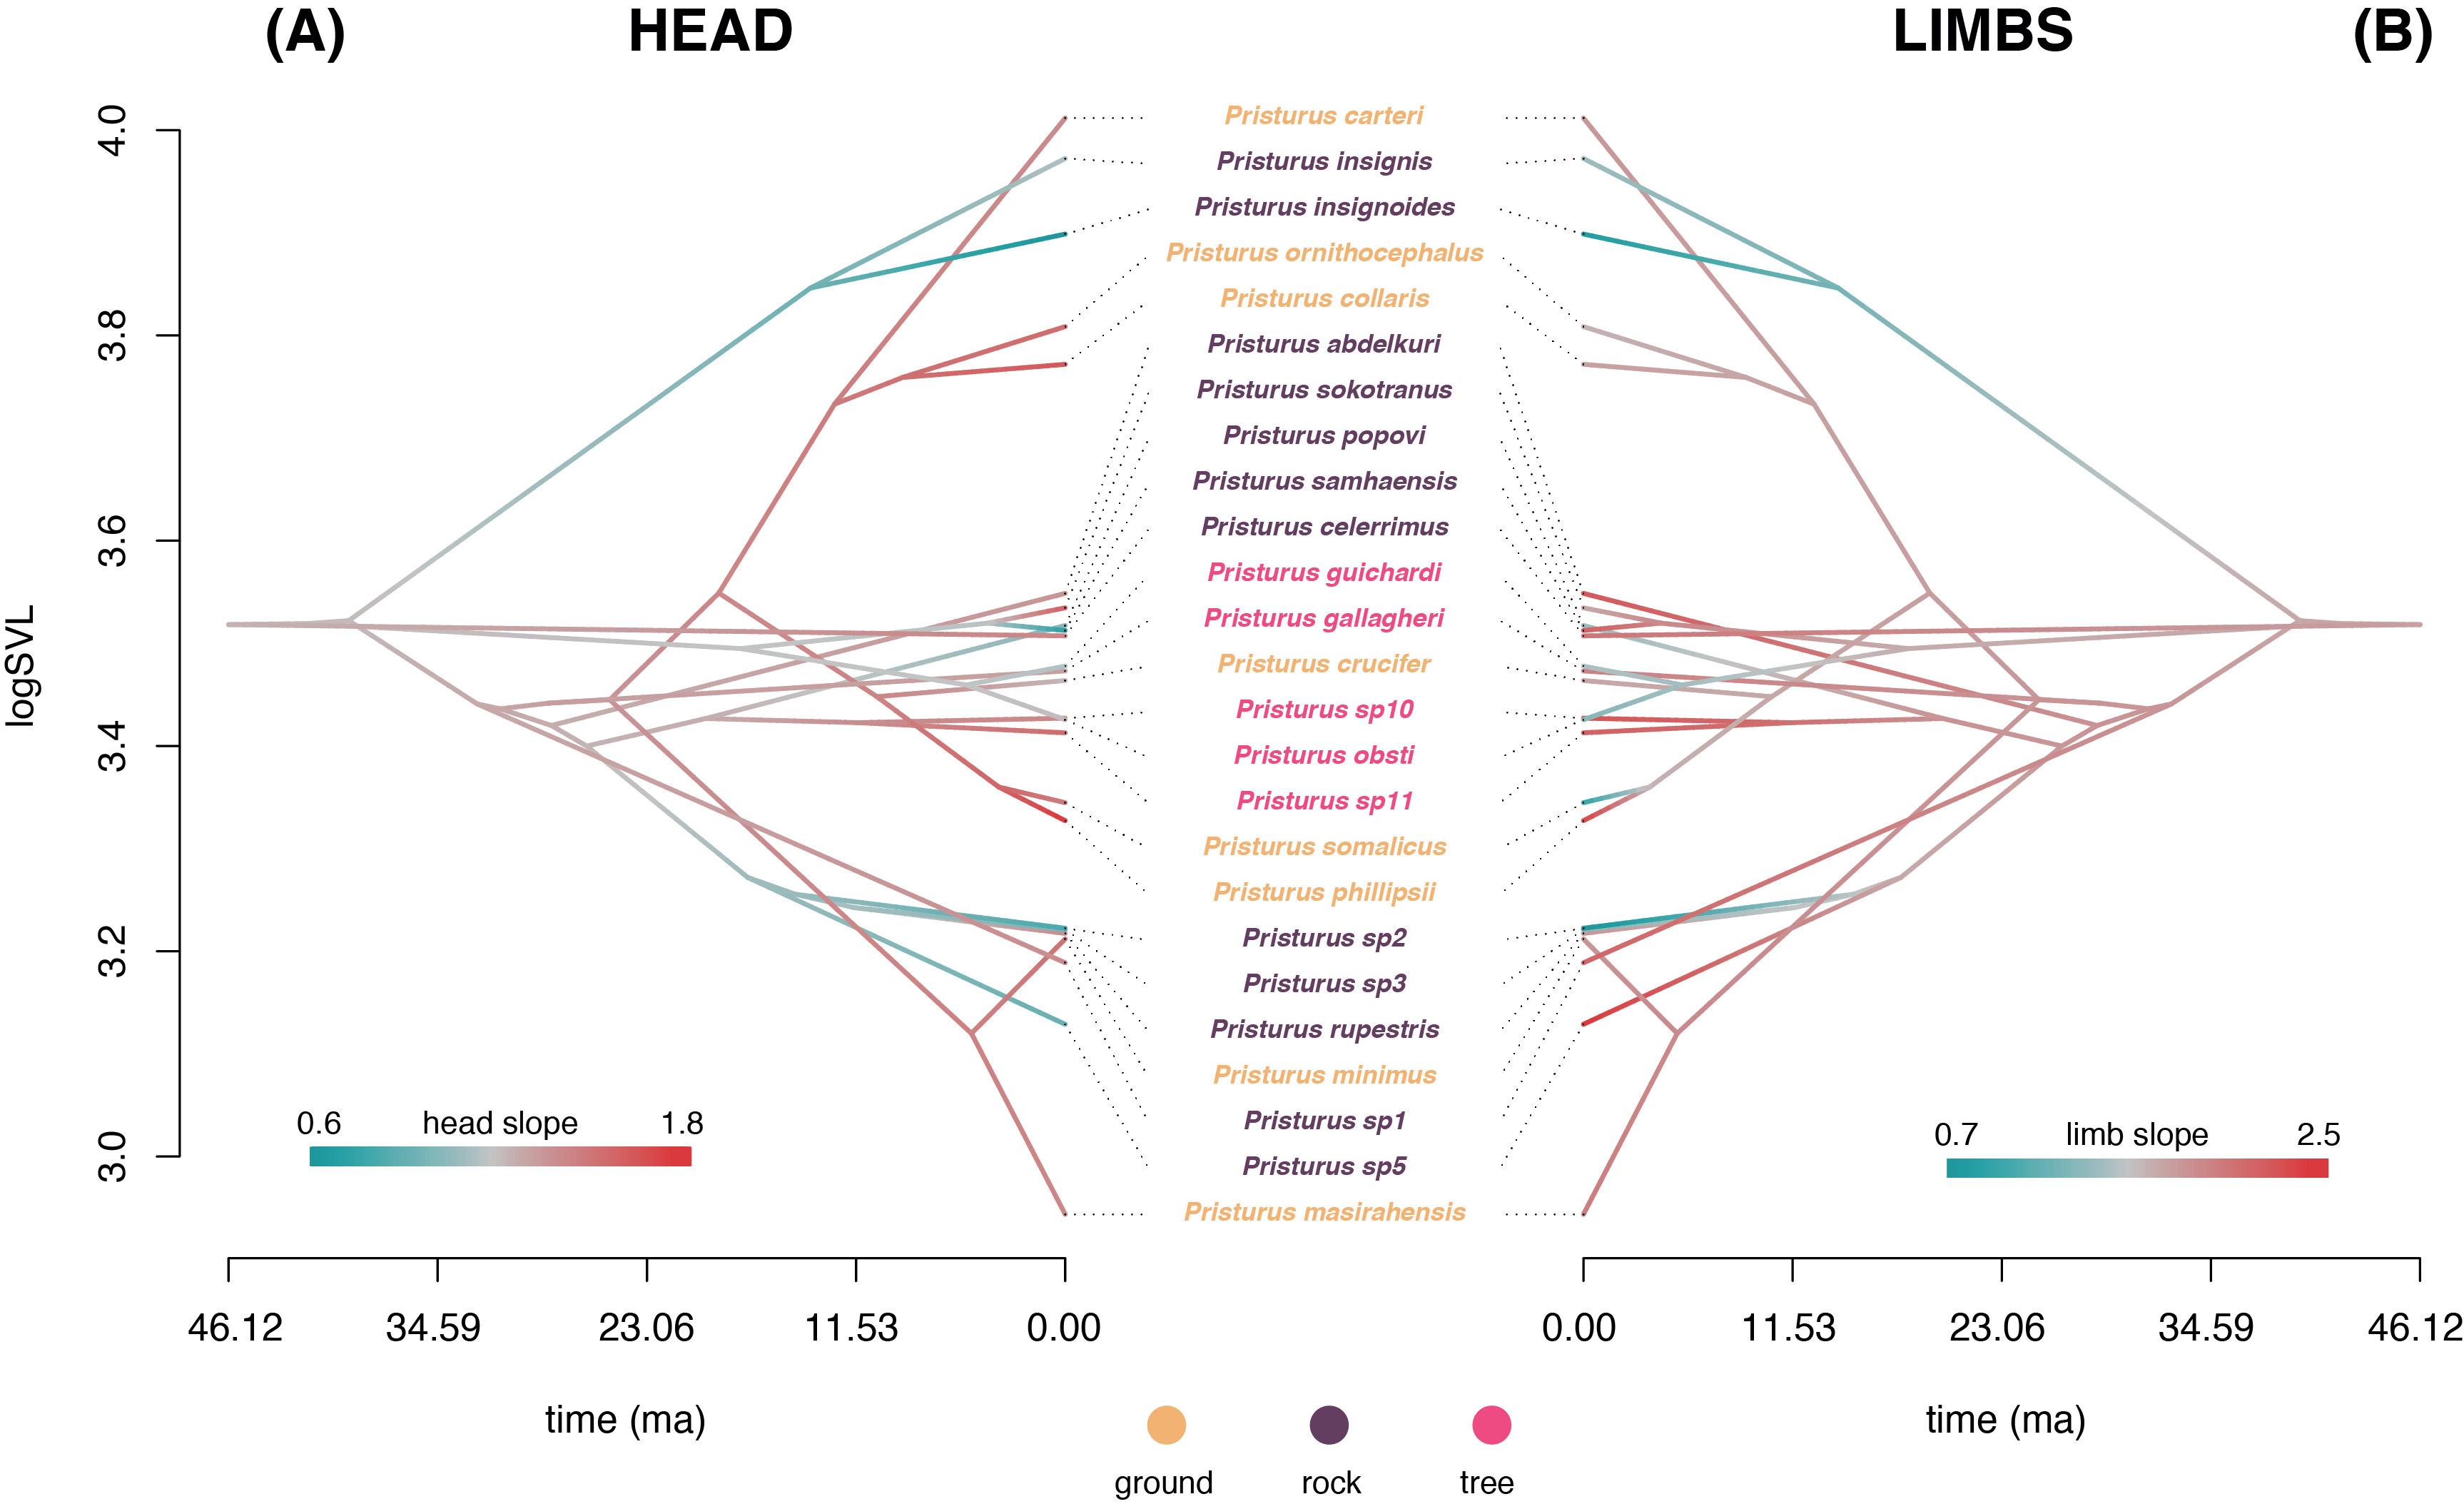
\includegraphics[width=1\linewidth]{Figs/figure_phenograms} \caption{Traitgrams showing the evolution of body size (SVL) through time based on the phylogenetic tree of \textit{Pristurus}. Colors represent an evolutionary mapping of regression slopes describing the relationship of (A) head morphology versus body size, and (B) limb proportions versus body size (see text for descriptions). Species names are colored by habitat use: rock (beige), ground (dark purple), and tree (magenta).}\label{fig:unnamed-chunk-5}
\end{figure}

\newpage

\begin{figure}
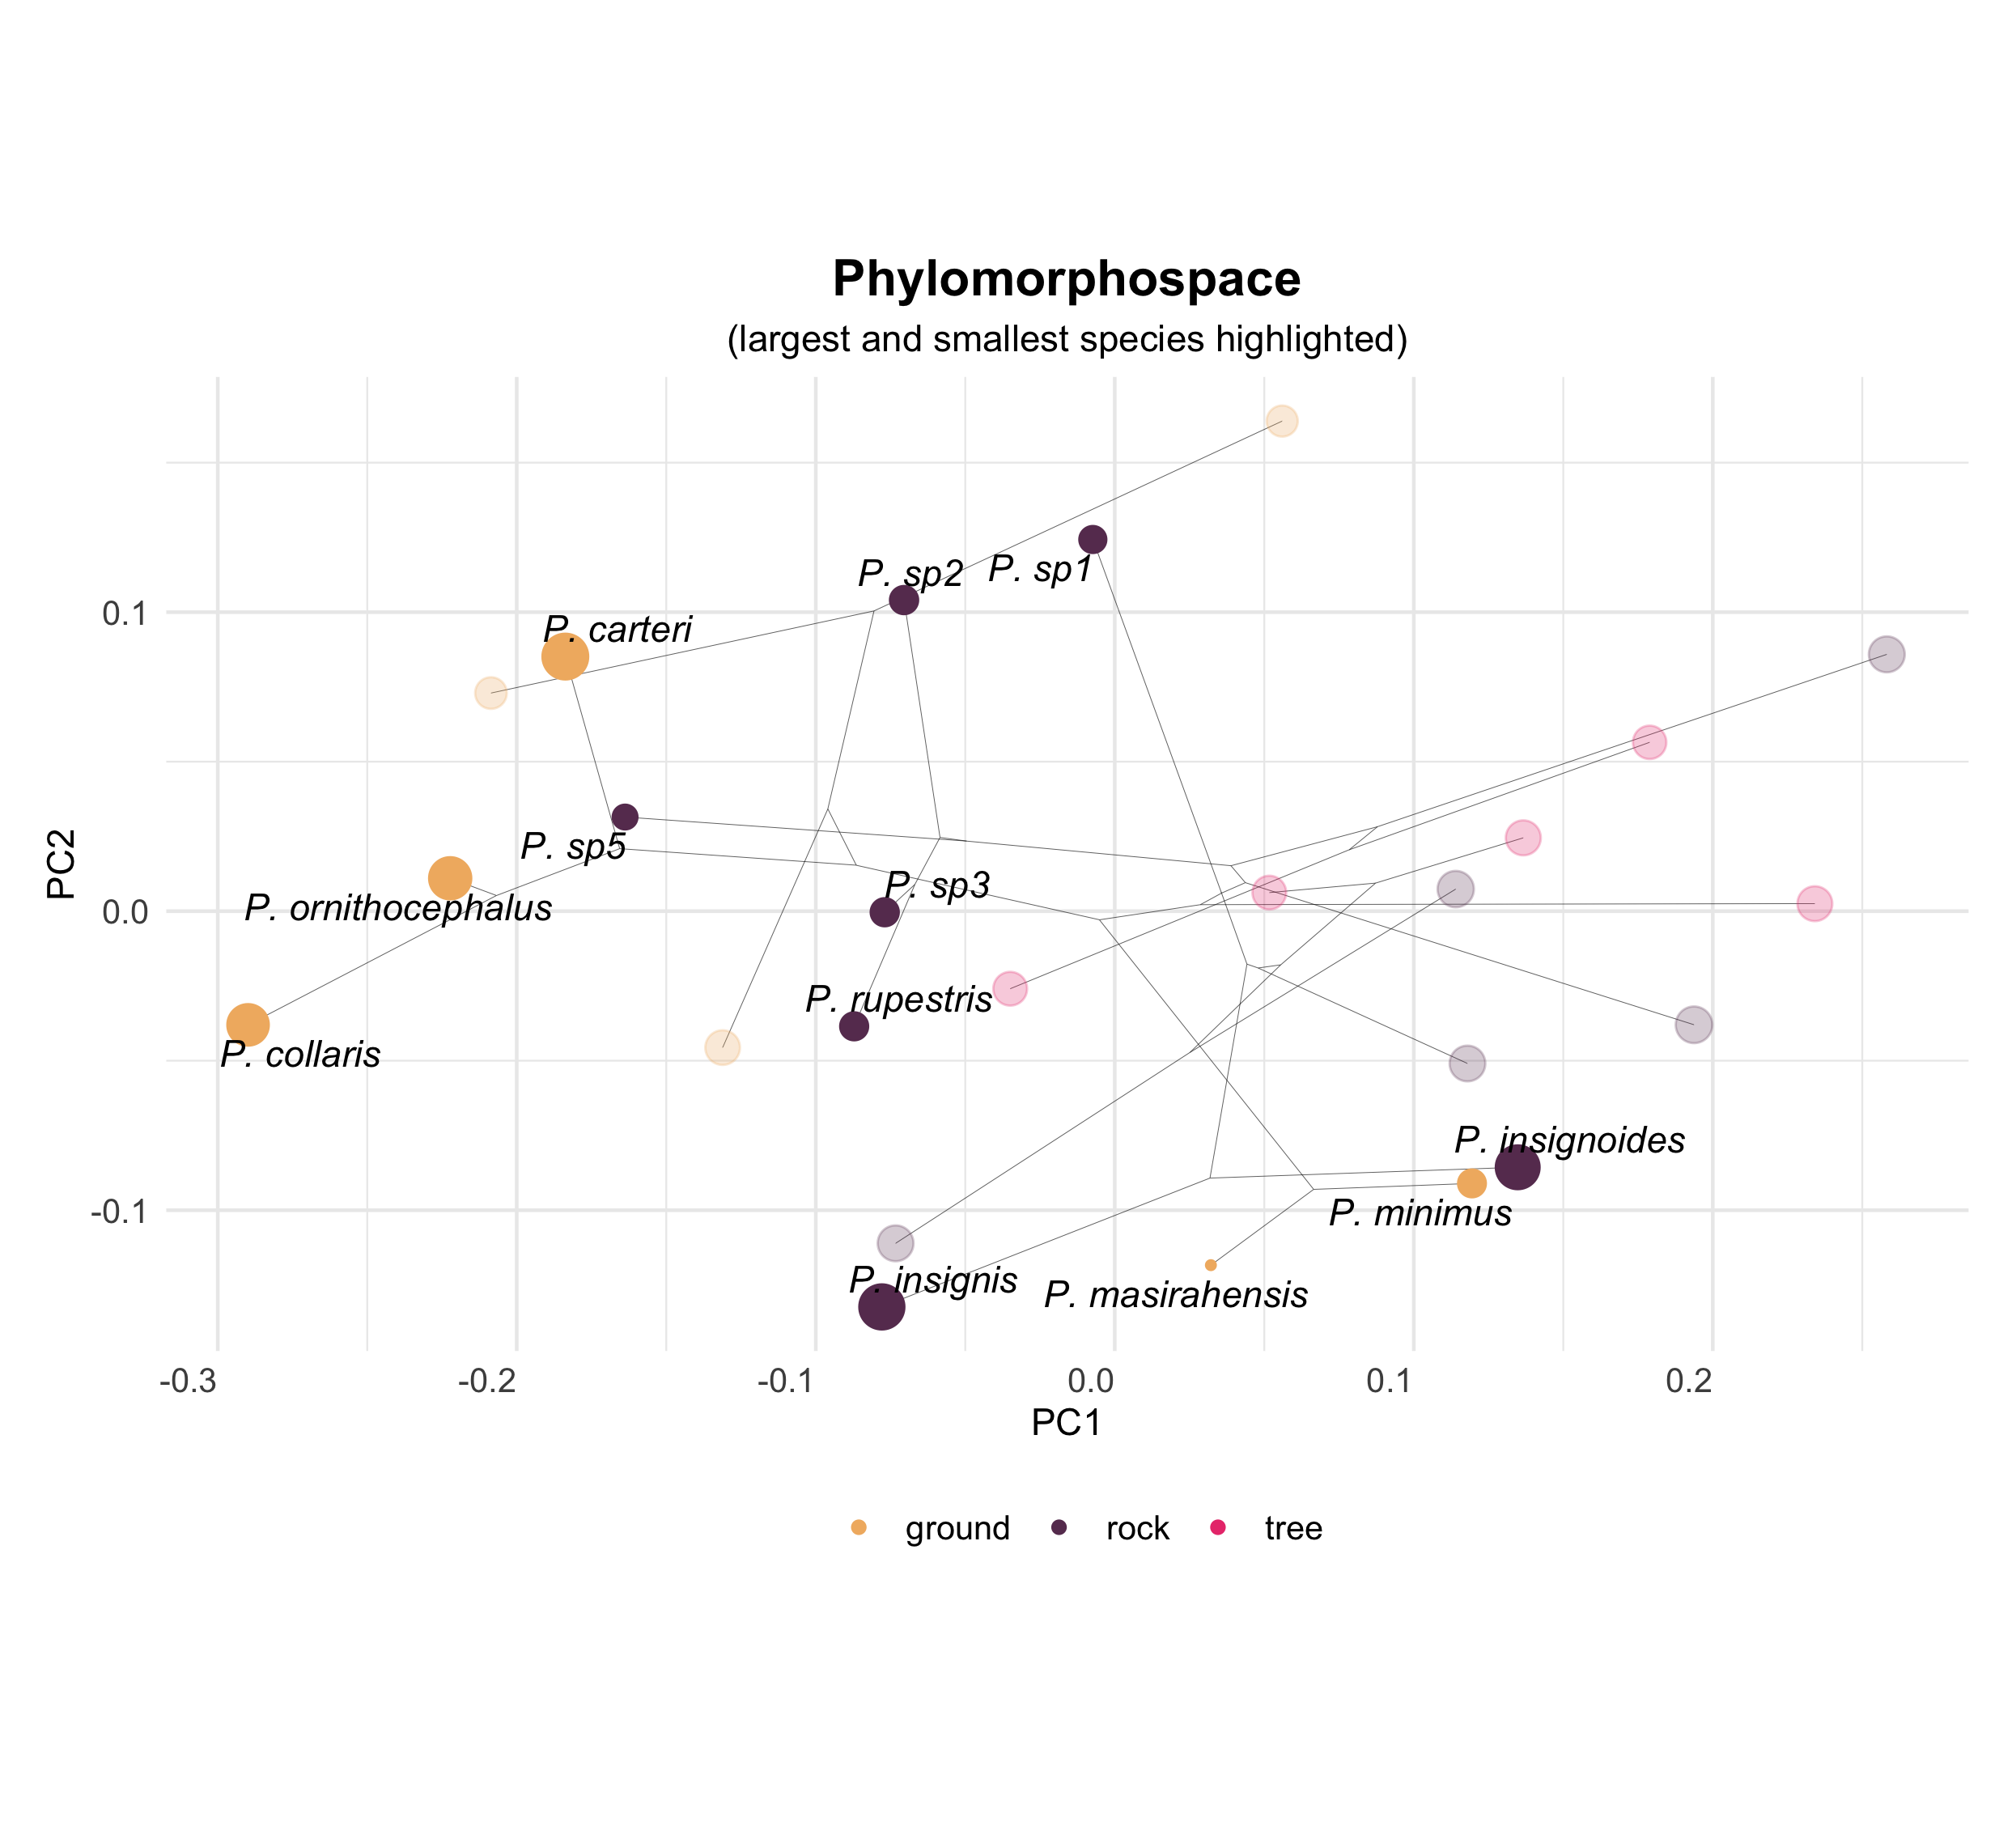
\includegraphics[width=1\linewidth]{Figs/phylomorphospace_large_small} \caption{Phylomorphospace of \textit{Pristurus}, based on residuals from a phylogenetic regression of body measurements on size (SVL). Species means are colored by habitat use: rock (beige), ground (dark purple), and tree (magenta). Large and small rock-dwelling and ground-dwelling are highlighted with darker colors to highlight their differentiation and relative positions in morphospace.}\label{fig:unnamed-chunk-6}
\end{figure}

\end{document}
